\section{Methodology}\label{sec:method}
\subsection{Shortest path}
Computing the shortest path between two vertices in an unweighted graph can be done using MS-BFS. 
In the current implementation by Singh et al., it is possible to determine the reachability of a node. 
However, to determine the shortest path, some form of state needs to be kept, such that it can be tracked how many hops have been done before reaching the destination node. 
Often, graphs have the small-world property, the distance between any two nodes is very small compared to the size of the graph~\cite{10.14778/2735496.2735507}. 
In addition, the shortest distance is always smaller than or equal to the diameter, the greatest distance between any two nodes, of the graph.
Therefore, in unweighted graphs, the size of the values needed to be stored in memory can also be relatively small. 
For every source node for which the shortest distance is computed, it will likely be enough to store the distance within 8 bits. 
Since the distance can never be negative, an unsigned 8-bit integer would suffice, in the case that the diameter of the graph is less than 255. 
However, we should care not to exceed this limit as the integer will overflow, causing it to wrap around to 0. 
Whenever that would happen we should copy the values into 16-bit or 32-bit unsigned integers to ensure no overflow errors occur.
This does reduce the efficiency of the MS-BFS algorithm compared to the reachability implementation. 
Computing the reachability only requires a 1-bit bool value per BFS, which is set to 1 in case the destination node is reachable, 0 otherwise. 
Using the AVX-512 operation, it is possible to execute 512 reachability searches at once. 
However, since computing the shortest path requires at least 8 bits to keep track of the distance, it will only be possible to execute $512/8 = 64$ BFS searches at a time. 
If we were to use 32-bit integers, only 16 BFS searches could be run.
Unsigned integers are preferred over signed, since the length of a path can never be negative, there is no need for negative integers. Denoting that a node is unreachable can be done by using \texttt{UINT\_MAX}~\cite{uint-max}. During execution, we keep track of the depth of the MS-BFS. Whenever this depth reaches \texttt{UINT\_MAX}, we know there is a chance for an overflow and make sure this is handled correctly.

To compute the cheapest path in weighted graphs, there are typically two algorithms that can be used, Dijkstra's algorithm using a Fibonacci heap and the Bellman-Ford algorithm.
% The Bellman-Ford algorithm has a worst-case time complexity of $O(|V|*|E|)$, however the expected runtime for large dense graphs is $O(E)$~\cite{DBLP:journals/dbsk/ThenGKN17}.
Then et al.~\cite{DBLP:journals/dbsk/ThenGKN17} propose a batched Bellman-Ford algorithm to compute the geodesic distance in weighted graphs. 
They find that the performance of the Bellman-Ford algorithm is 3-10x higher compared to a batched variant of Dijkstra's algorithm~\cite{DBLP:journals/dbsk/ThenGKN17}.
Therefore, we will first look to implement the batched Bellman-Ford algorithm proposed by Then et al. as shown in Algorithm~\ref{alg:batched-bellman-ford}. 
Implementing a batched version of Dijkstra's algorithm will be more complex.
During the batched version multiple instances of Dijkstra's algorithm will run, each having its Fibonacci heap.
Given that each heap will be of a different structure, the effectiveness of possible SIMD instructions will be reduced. 
Therefore, it is not likely that a batched version of Dijkstra's algorithm will outperform the batched version of the Bellman-Ford algorithm. 
To test the performance of the implementations we will be using the LDBC Graphalytics benchmark~\cite{DBLP:journals/pvldb/IosupHNHPMCCSAT16}, which is designed to test various algorithms such as single-source shortest path (SSSP) and BFS.
Additionally, we will be using the LDBC Social Network Benchmark~\cite{DBLP:journals/corr/abs-2001-02299} to further test the performance of the implementations.


\subsection{Shared hash join}
Queries can contain multiple expensive joins which are in essence identical. This also happens in graph-like queries, where it is common to join the vertex table twice on the edge table. Once for the source of the edge, and once for the destination of the edge. 

In the current state of DuckDB, for each join a hash table is built from the smaller table. 
However, this is wasteful in the case where queries containing multiple join operations have identical sinks. 
For example, there exists a vertex table \textit{Person} containing the column \texttt{person\_id}, and an edge table \textit{Knows} containing the columns \texttt{person1\_id} and \texttt{person2\_id}. These tables are used to build a CSR representation for the edge table. 
Thus, it is necessary to perform two joins, namely $\texttt{person1\_id} \Join \texttt{person\_id}$ and $\texttt{person2\_id} \Join \texttt{person\_id}$. 
In this case, the right side is identical in both joins. 
See Figure~\ref{fig:physicalplanhashjoin} for the relevant part of the physical plan of this example query.
An optimization is to build this hash table only once, and reuse it for any identical joins containing the same sink. 
This will eliminate the need to build the same hash table multiple times.

\begin{figure}
  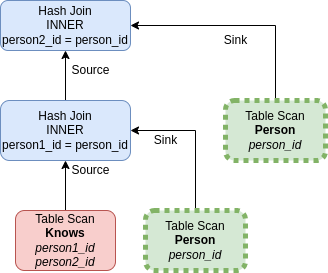
\includegraphics[width=0.6\linewidth]{figures/physicalplan-shared-hash-join.png}
  \caption{Example of a duplicate sink state in the physical plan}
  \label{fig:physicalplanhashjoin}
\end{figure}

The plan for the shared join optimization is to make the sink shareable between multiple pipelines in the case where the joins are identical. 
This will eliminate the need of building multiple identical hash tables since they can be reused. 
During the building phase of the pipelines, we will save all join operations we come across in combination with its respective pipeline. 
In the case where a duplicate join is encountered will the sink state of that pipeline be shared with the sink state of the pipeline seen earlier. 
In addition, the dependency of the parent pipeline on the current pipeline needs to be changed.
The optimization can not be performed on FULL or RIGHT joins. 
For these joins a state needs to be kept for the hash tables to see if a particular value has been accessed or not.
This access may vary between joins, and thus will result in different states. 
Therefore, the hash table cannot be reused for these types of joins. 

% Additionally, a case where the two joins make use of the same table but with different columns has to be taken care of.
% A solution would be to use the union of these columns to build the hash table. 



% A similar optimization can be performed for identical table scans. 
% Table scans are unique to a pipeline, and thus it is not known for other pipelines which tables have been scanned. 
% An optimization is to share table scans in case multiple identical ones are encountered in the query, removing the need for multiple table scans.

% A case needing to be considered with both joins and table scans is when 


% In DuckDB, an optimization rule will be added called 'Shared Hash Join'. During the optimization phase, the rule will be used to identify all tables used in combination with a join statement and store the table name in the client context of the query. 
% It is not sufficient to store the alias of the table (In Listing~\ref{lst:duplicatejoin} p, p2, and k), since these are likely different even if the same table is used.
% Storing only the table name can work initially, though more information is needed, such as possible filters applied on any of the joins.

% During the logical planning stage, a tree of basic logical query operators is built. 
% Examples of these are \textit{get} or \textit{comparison join} operators. 
% The get operator has no children, since this is the instruction to retrieve a specific table. 
% A comparison join operator has two children, the two operators which will be joined at a later stage. 

% \begin{figure}
%   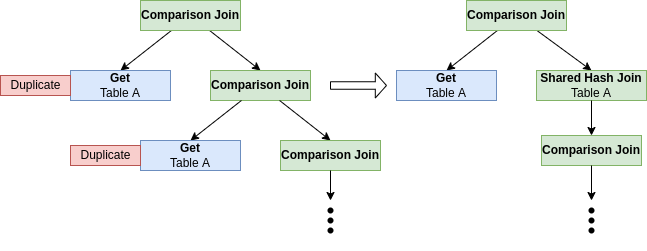
\includegraphics[width=0.75\linewidth]{MSc-thesis/figures/Sharedhashjoinlogicalplanner.png}
%   \caption{Logical query operator tree optimization}
%   \label{fig:sqlpgqgql}
% \end{figure}

% During the optimization phase, we will identify the tables on which joins are performed. 
% If we identify a join on a table that is seen previously, i.e. an identical join, we will swap the comparison join operator for a shared hash join operator. 
% Once the tree has been traversed, all duplicate joins will have been identified and been replaced by the shared hash join. 

% After the optimization, a physical plan is created from the resulting query tree.
% Within this plan, every join has a unique state containing among other things the hash table. 
% For the shared hash join, this state has to be shared between multiple join operations. 
% In addition, other operations could be dependent on the outcome of the join operation. 
% When using the shared hash join, we should correctly identify the dependencies of the join operator and link these to the shared hash join operator instead.



% This is important since it is not possible to use a copy of a hash table that is yet to be built.
% Within the physical planner, it should be checked whether the hash table for a given table has been built. 
% If it is, we do not build a new hash table, instead, we point to the already build hash table. 
% If it is not yet built, we will proceed as normal and build the hash table. 

% A possible edge case is when the joins are very similar, but each retrieve different columns. 
% In this case, the union of columns should be taken such that both tables have all columns required for the query. 
% Another case is when a filter is applied on one of the joins, but not on the other, otherwise identical, joins.

% In some cases, the various joins make use of hash tables with identical contents. 
% In this case, it is wasteful to build these duplicate hash tables more than once. 
% Instead, it is better to build the hash table once, and allow it to be reused by the other joins. 
% A specific example where this is the case is during the building of the CSR-like data structure for SQL/PGQ queries, as described by Singh et al.~\cite{sqlpgq-duckdb}.

%  However, in the case of Listing~\ref{lst:duplicatejoin}, the multiple joins will result in multiple identical hash tables for the smaller of the two tables in the join. 
% The optimization identified is to only build the hash table once, and allow it to be reused when duplicate joins are found.


In DuckDB, unit tests can be written using the \textit{SQLLogicTests framework} to test the correctness of the implementation~\cite{duckdb-testing}. 
Assuming that the implementation works correctly, we will be testing the performance of the optimization using the CSR creation queries used by Singh et al.~\cite{sqlpgq-duckdb}. These queries contain a duplicate join on the vertex table.
% Additionally, of the TPC-H benchmark, query 21 (see Listing~\ref{lst:tpc-h-query21}) contains a duplicate join that can be used to test the performance. 
By performing tests with and without the optimization, we should see that the queries using the optimization have a lower run-time. 

% \begin{lstlisting}[caption=TPC-H Query 21, label=lst:tpc-h-query21] 
% -- TPC-H Query 21

% SELECT
%     s_name,
%     count(*) as numwait
% FROM
%     supplier,
%     lineitem l1,
%     orders,
%     nation
% WHERE
%     s_suppkey = l1.l_suppkey
%     AND o_orderkey = l1.l_orderkey
%     AND o_orderstatus = 'F'
%     AND l1.l_receiptdate > l1.l_commitdate
%     AND EXISTS (
%         SELECT *
%         FROM lineitem l2
%         WHERE
%             l2.l_orderkey = l1.l_orderkey
%             AND l2.l_suppkey <> l1.l_suppkey
%     )
%     AND NOT EXISTS (
%         SELECT *
%         FROM lineitem l3
%         WHERE
%             l3.l_orderkey = l1.l_orderkey
%             AND l3.l_suppkey <> l1.l_suppkey
%             AND l3.l_receiptdate > l3.l_commitdate
%     )
%     AND s_nationkey = n_nationkey
%     AND n_name = 'SAUDI ARABIA'
% GROUP BY
%     s_name
% ORDER BY
%     numwait desc,
%     s_name
% LIMIT 100
% \end{lstlisting}






% This section will provide details on how the research topics will be tackled and evaluated. A small planning is also provided. 

% \subsection{How will the problems be tackled}
% Work on integrating SQL/PGQ into DuckDB is currently being done in a publicly available GitHub repository~\cite{sqlpgqduckdbrepo}. Any further work done on integrating SQL/PGQ in DuckDB will be performed in this repository. In the current implementation, reachability has been implemented as a User Defined Function (UDF) in DuckDB. Creating UDFs will likely be the optimal way of implementing functions with which the path length and the actual path can be retrieved. 
% Once the UDFs have been implemented they should be benchmarked using the LDBC Graphalytics Benchmark~\cite{DBLP:journals/corr/abs-2011-15028}. This open-source industrial-grade benchmark consists of several deterministic algorithms for graph analysis and provides a fair comparison to other graph-based systems~\cite{DBLP:journals/corr/abs-2011-15028}. 

% Work on optimizing the hash tables will also be done in the same repository~\cite{sqlpgqduckdbrepo}. However, before the optimization can be implemented, it should be discussed with the development team of DuckDB to decide on the optimal way to implement it. Once implemented, the optimization should be faster consume less memory, as only one hash table needs to be built instead of 2 or more. The optimization can be compared to a version without the optimization to assess its effectiveness. Apart from the optimization, as much as possible between the two systems should be the same to provide a fair comparison.  

% To the best of our knowledge, currently, no standard test suite exists to analyse the performance of the SQL/PGQ integration in a relational database. Therefore, one of the goals of this thesis is to create such a test kit. The kit should involve a wide variety of graph patterns and navigational expression queries to provide a comprehensive test. These tests should then be benchmarked and compared to other GDBMSs such as Neo4j~\cite{Neo4j2018}, TigerGraph~\cite{tigergraph}, and GRainDB~\cite{graindb}.



% see Listing~\ref{lst:duplicatejoin} for example. This example contains a triangle query where the data of \textit{knows} and \textit{person} tables are joined multiple times on the same keys.
% \begin{lstlisting}[caption=SQL query containing identical joins, label=lst:duplicatejoin]
% SELECT p.pid, p2.pid 
% FROM person p, knows k, person p2, knows k2, person p3, knows k3 
% WHERE p.pid = k.pid 
%     AND p2.pid = k.kid 
%     AND p2.pid = k2.pid 
%     AND p3.pid = k2.kid 
%     AND p3.pid = k3.pid 
%     AND p.pid = k3.kid
% \end{lstlisting}


\subsection{Planning}
See Table \ref{tab:planning}.


\begin{table}[]
\begin{tabular}{|l|l|}
\hline
\textbf{Month} & \textbf{Goals}                                                                                                 \\ \hline
February       & \begin{tabular}[c]{@{}l@{}}Work on literature study \\ Start on optimization shared hash tables\end{tabular}   \\ \hline
March          & \begin{tabular}[c]{@{}l@{}}Work on optimization hash tables\\ Start on shortest path using MS-BFS\end{tabular} \\ \hline
April          & \begin{tabular}[c]{@{}l@{}}Finish optimization hash tables\\ Finish shortest path and experiment\end{tabular}  \\ \hline
May            & \begin{tabular}[c]{@{}l@{}}Start on cheapest path using \\batched Bellman-Ford / Dijkstra\end{tabular}         \\ \hline
June           & \begin{tabular}[c]{@{}l@{}}Finish cheapest path \\ Start on experimenting\end{tabular}                         \\ \hline
July           & \begin{tabular}[c]{@{}l@{}}Finish up experimenting\\ Finish up writing\end{tabular}                            \\ \hline
\end{tabular}
\caption{Initial planning
}
\label{tab:planning}
\end{table}




